\documentclass[12pt,a4paper]{article}
\usepackage{ucs}
\usepackage{caption}
\usepackage[latin1,utf8x]{inputenc}
\usepackage{amsmath}
\usepackage{caption}
\captionsetup{font=small,labelfont=bf}
\usepackage[danish]{babel}
\usepackage[rmargin=3cm,tmargin=3.3cm]{geometry}
\usepackage{listings}
\usepackage{color}
\setlength{\parindent}{0pt}
\setlength{\parskip}{1ex plus 0.5ex minus 0.2ex}
\usepackage{graphicx}
\usepackage{fixltx2e}


%insert links
\usepackage{hyperref}
\usepackage{fancyhdr,lastpage}	
\pagestyle{fancy}


\definecolor{mygreen}{rgb}{0,0.6,0}
\definecolor{myblue}{rgb}{0,0,1}
\definecolor{myyellow}{rgb}{0.7,0.7,0}
\definecolor{myblack}{rgb}{0,0,0}

\lstset{
	breaklines=true,
	numbers=left, 
	commentstyle=\color{mygreen},
	stringstyle=\color{myyellow},
}

%header
\lhead{ 
	Embedded Systems \\
	02131 \\ 
}
\chead{ 
}
\rhead{ 2 October, 2012 \\ \bigskip  }

%Footer
\lfoot{
	\rule{\textwidth}{0.1mm}\\
}

\cfoot{}
\rfoot{\ \\ \scriptsize{Side \thepage\ af \pageref{LastPage}}}

\begin{document}

%Forside
\begin{titlepage}
	\begin{center}
		\vspace*{13\baselineskip}
		\huge
		\bfseries
		Embedded Systems\\ 
		\ \\
		02131 \\[5\baselineskip]

		\normalfont
		\Large
		R-peak detection!\\	
		2013

		\small
		\vfill
	\end{center}	
	\begin{flushleft}
		Jakob Welner, s124305\\
	 	Jacob Gjerstruo, s113440\\
	\end{flushleft}
\end{titlepage}

\ \\
\section*{Abstract}
The task of this assignment was to develop an Electro-Cardiogram (ECG) scanner using the Pan-Thomkins QRS-Detection Algorithm, and then implement this algorithm in the language C. Using this algorithm, a program has been created that can determine a persons heartbeat and give warnings when either the intensity or the heartrate falls below a certain threshold. The program has initially been based on sample data gathered from an ECG scanner and read from a file. However, care has been taken in making it easy to replace the data source at a later point. 
All algorithms provided by the assignment were implemented successfully although certain issues persisted.

\thispagestyle{empty} 
\newpage

%Table of Contents
\tableofcontents
\thispagestyle{empty} 
\newpage

%Reset pagecount
\setcounter{page}{1}

%Alm. sider
\ \\
\section{Introduction}
	This report will investigate the Pan-Thomas QRS detection algorithm, more specificly, if it is possible to implement this algorithm into the company Medembed's next product, which is a wearable ElectroCardioGram (from now on simply called ECG) scanner.\\
	The algorithm will be implemented in the programming language C, and this report will discuss the following topics: Data acquisition, implementing filters, implementing the peak-detection algorithm, outputting the data to the user and finally, an analysis of the algorithm in terms of power consumption, speed (clock cycles per second) and code size.\\
	For the purpose of this report, we will only implement the C program, and will simulate the data acquisition in real time through data files. Furthermore, the program will be run on an all-purpose processor, whereas in the final product of Medembed, a dedicated processor with limited resources will be used.\\
\\
\subsection{Requirements}
Below follows a list of functional and non-functional requirements:\\

\textbf{ Functional requirements for the application:}
\begin{itemize}
	\item Data acquisition in simulated real-time
	\item Implementation of the 5 filters
	\item Implementation of the R-peak detection
	\item Output of relevant data to the user, based on the algorithm
	\item An analysis of our implementation as well as the critical parts, runtime and memory requirements.
\end{itemize}
\textbf{Non-functional requirements for the application:}
\begin {itemize}
	\item The programming language used for this is C
\end{itemize}

\section{Theory}
 	In order to initiate the structure- and design-process of the program, a number of questions needed to be answered first:\\
 	
 	\begin{enumerate}
	\item How should the real-time data acquisition be simulated?
	\item How should the filters be integrated?
	\item How should the R-peak detection be integrated?
	\item Which data would be relevant for the user, and how should it be shown?
	\item How do you determine the critical parts?
\end{enumerate}

\subsection{Problem 1: Data acquisition}
	As specified in the introduction, the dataset used was only sample data and not current readings. To ensure that the program would work on live data as well as samples, a method for reading single datapoints sequentially was implemented, thus simulating real data acquisition. Loading single datapoints while needing to handle both the current data as well is the biggest challenge when it comes to data acquisition.\\
	
\subsection{Problem 2: Implementation of Filters}
	To use the QRS-algorithm to it's full extent, the raw data should go through a list of 5 filters, cleaning up the data, amplifying peaks and removing unwanted noise. 4 of these filters use multiple datapoints simultaneously, both current and previous samples, while lowpass and highpass use previous samples from their own filtered output. To allow for easy access to the saved datapoints at different given points in time, the readData buffer method was extended to include a time offset input value. This would work as an index for the data array, though combined with the built-in counter, would amount to a number of steps back in time. ReadData(buffer, 0) would read latest pushed data from 'buffer' and readData(buffer, 3) would read the data stored 3 loops earlier. Furthermore, passing pointers of buffer structs to the buffer-methods allowed to change the provided buffers inplace\\
\\	
Having extended the method successfully while simply returning 0-values when requesting data before 1st loop, implementing the filters was a matter of writing the equations from the assignment and requesting the appropriate datapoints directly.
	Allowing lowpass and highpass to read from their own output was then elementary. Passing a pointer of the input- and another of the output-buffer would give each filter access to read/write on both\\

\subsection{Problem 3: Implementation of R-peak detection}
	Once all the filters had been implemented, the actual QRS-algorithm was the next step. The QRS-algorithm would be the one to determines what consitutes a heartbeat, and how to analyse it. Furthermore, it would serve to determine how R-peaks are identified, and after each peak, it will update certain variables to ensure the heartbeats are tracked correctly. These variables will be the ones determining when a heartbeat is certain than a threshold, and if it is, this peak is referred to as an R-peak. Once an R-peak has been determined, data is updated further to classify the next peaks as either heartbeats or noise. This algorithm, however, introduces three challenges - how to determine whether the patient simply has irregular and/or weak heartbeaks or whether the patient is having a heart attack; and how to ensure that every heartbeat is detected correctly. The final challenge was that the algorithm requires that all peaks are stored, and as there is no knowing how many peaks will be found, a list of flexible length was needed.\\

\subsection{Problem 4: Relevant data}
	The requirement states that the program must show at the very least the value of the latest R-peak that was detected, and also, it must show when this R-peak happened, plus the patients pulse. Furthermore, the patient must be given a warning of the R-peaks value is less than 2000 (as this is a sign of an impending heart attack) and finally, if 5 successive RR-intervals has missed the RR- LOW and HIGH values, these must be shown. However, how these data are to be shown has not been defined, and therefore must be specified.\\
	\\
	There are several ways to show these data, of which the simplest is to make a text-based screen with the information necessary, and keep this screen updated in real-time, showing the data as we calculate them. Alternatively, the data can be plotted and shown in a graph, or one could combine these two, giving both a graph that keeps getting updated in real-time, as well as text-based information.\\

\subsection{Problem 5: Critical parts}
	The final issue that was to be clarified is the critical parts of the program. Here, there are three points to discuss, memory requirement, time consumption and power consumption.\\
	Memory requirement is important as the bigger the program is, that is, the more memory it requires, the more physical memory must be implemented into the final device, and therefore, the device will become larger and more cumbersome to wear. Furthermore, more memory also means that the device becomes more power-consuming.\\
	Time consumption is important as the device must be able to read at least 250 data points a second, and if the functions are very time consuming, a stronger processor is needed that requires more power. Furthermore, it is also important that the processor used does not process the data too fast, either, as this will mean that the processor will idle and use power for nothing, meaning a smaller processor can be used that requires less power.\\
	Power consumption is important as it determines how often the user must either recharge the battery or be issued a new battery.\\
	
\section{Design}
	When designing the program, it was quickly decided that multiple files should be used for easier readability. Each file would consist of functions concerning a single topic, ie: the filter.c would contain filters-related methods only. The files used are: filter.c, buffer.c, main.c, RRhandling.c and sensor.c.\\
	\\
	Furthermore, it was decided that the data from each filter, as well as the raw data, would each be stored for a set amount of time. An amount of 33 samples was choosen given that no filters request values older than 32 readings before current. Allocating more memory would therefore be a waste and having less samples stored, would break the algorithm.\\
	\\
	To handle the actual data a buffer was created. The mainloop would then run through the data-set, scanning in a point and passing it to the buffer. The buffer would then handle storing and retrieving data through a struct type and 4 dedicated buffer-methods. This array would then be passed on to the filters which would sample individual datapoints, apply the appropriate math and update the buffer-values accordingly.
	\\
	\\
	%write something about R-peak detection design decisions


\section{Implementation}
\subsection{Core structure}
The support the overall functionality and readability of the program a core structure needed to be laid out. First and foremost the dataflow should be handled. Data coming from the sensor should be stored for later processing. Storing such data could be handled in many ways but it was decided to construct a type of buffer which would allow for easy pushing and pulling data, while only keeping a certain amount of history.
The buffer will also keep track of where in the array the data is, and should it exceed the size of the array, it will return to the first place in the array (indexed to 0) and overwrite the data there.
In order to get around returning huge lists of data between functions, the buffer would instead update the input variables in-place through pointers.
Last bit of the core was to set up a list for containing validated R-Peaks. Given that all R-peaks should be saved, the list would be of an arbitrary length. While the C-language is very poor at handling arrays with ill-defined length, a linked list was used instead. The linked list works by defining a Struct type which contains a variable pointer to another struct of the same type. Adding each R-peak as a new struct instance while assigning it a pointer to the previous r-peak struct, would allow for a so-called linked list of arbitrary length.

\subsection{Real-time data acquisition}
	As described, the program must acquire the data and calculate in real-time. To ensure this simulation, the program loads one data point, then passes it and the corresponding array to the one filter at a time before it finally passes it to the peak detection and subsequently, to the R-peak detection. Once all these calculations have been done, it loads in a new data point and restarts through a while loop.\\
	This while-loop will run through the entire data-set, and will not stop before it reaches the end of the file (in the finished product, it will of course run until the battery runs dry).\\
	\\
	Furthermore, it was found that in order to always keep a list of previous samples while maintaining easy access to their relation to the current data, structs and methods could be used to create a buffer - more specificly, this buffer was implemented using a struct containing an integer array as well as a counter. Using a list of simple method-functions to handle pushing of data as well as reading, a simple circular First In First Out (FIFO)-list was created.
	
	Therefore, the combination of the while-loop that runs forever, and the continual loading and subsequent calculations through the buffer solves the challenge of real-time data acquisition.\\

\subsection{Implementation of Filters}
	The first implementation of the filters were simply done with strict if/else sentences. However, this was changed to using an adaptive index that, should it reach negative values, moves to the end of the array instead. This way, the program should never encounter data under- or overflow, and thereby, the first of the challenges were solved.\\
	The second challenge, to ensure the correct transfer of data from one filter to another, was solved by using two arrays, one for the raw data and one for the filtered data. Each array is then passed to the next part of the program, ensuring all filters have both raw and processed data to be operated on, as 4 of them requires.\\
	\\
	Therefore, the use of two arrays and an adaptive index solves the challenge of the implementation of the filters.\\
	
\subsection{Implementation of RPeakDetection}
	When implementing the RPeakDetection, the filtered data was run through a simple local-maxima detection and saved in a new list. As noted in Problem 3 - Implementation of RPeakDetection, this list needed to be of flexible length, and looking at the different options for implementing such a list, the decision fell on linked lists through structs. This struct contains a 'next'-variable with a pointer to the same type of struct. For each new instance of the struct, the intern next-value is set to point at the previous struct, thus linking the two together. 
	Having implemented the linked list, 3 variables were added to the struct; VALUE, CLOCK and TYPE. Accordingly, these would contain the signal-strength of the peak, at what time the sample had occurred and what type it had been classified as. TYPE was handled as integer values where -1 meant noise-peak, 0 meant a local-maxima peak, 1 meant an R-peak and 2 meant a regular R-peak. This would allow for all the peaks to be stored in a single list while enabling searching through the list and filtering for several types at a time while comparing results. 
	After this had been set up, the algorithm for determining r-peaks was implemented. To allow a few samples to appear before trying to enhance variable values, a MINSAMPLES value was defined.\\
	\\
	Therefore, the combination of the algorithm and the linked list solves the challenges of the implementation of RPeakDetection.
	
\subsection{Relevant data}
	To display the relevant data, a simple text-based display was created. This would show the required information, that is, the value of the latest R-peak, the time of the R-peak, the patients pulse. Furthermore, it will also display the warning and the RR-LOW and RR-HIGH values if 5 RR-intervals has been missed.\\
	\\
	Therefore, the challenge of the relevant data has been solved.
\subsection{Critical parts}
	As mentioned in the theory, the three critical parts of the program is memory consumption, power consumption and time consumption. The program was initially tested on a machine running a powerful all-purpose Intel Core i7-2630M CPU with a clock speed of 2GHz and consumes a maximum of 45 Watt. \\
	As can be seen on the figure below, the processor manages to process 10.000 data points on 0.02 miliseconds which is far more than what is required (250 data points per second).\\
	In terms of power, as said, the current processor on which the program was tested consumes a maximum of 45 Watt. This can be reduced by either reducing the calculation-power of the processor (clock frequency) or the size of the processor.\\
	In regards to size....	
	\begin{figure}[h!]
		\centering
			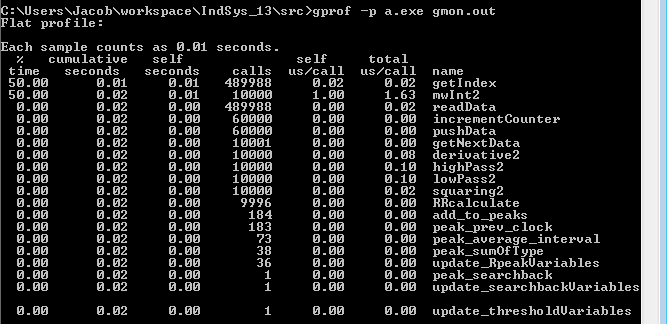
\includegraphics[width=1\textwidth]{Screenshots/time_result.png}
		\caption{The table above shows the time spent in the various filters in our program. It should be noted that this profiling was done without code optimization.}
		\label{time_result}
	\end{figure}
	
\section{Results}
	Figure 2 shows a screenshot of the output from the RPeak detection algorithm. It shows the output, both when the user has a normal heartbeat (the first part), the warning when the users heartbeat suddenly drops dangerously low, and the warning when the user has a heart attack. Furthermore, it always shows the heartrate (in Beats Per Minute (BMP)), as well as the RPeak values and the time since the last RPeak.
	
	
	\begin{figure}[h!]
		\centering
			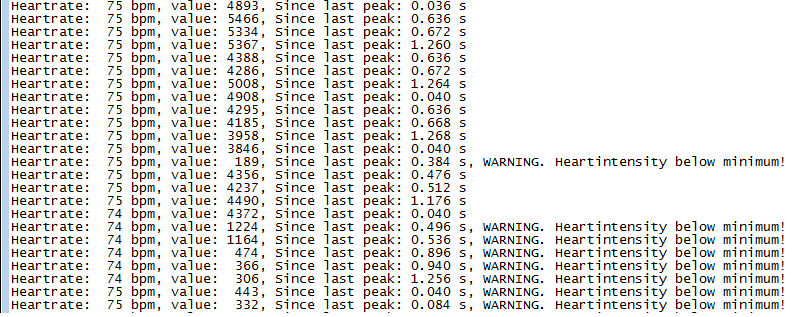
\includegraphics[width=1\textwidth]{Screenshots/RPeakDetection_result.png}
		\caption{A screenshot of the output of the RPeak detection.}
		\label{RPeakDetection_result}
	\end{figure}
\subsection{Test results of filters}

\begin{figure}[h!]
%  \centering
%    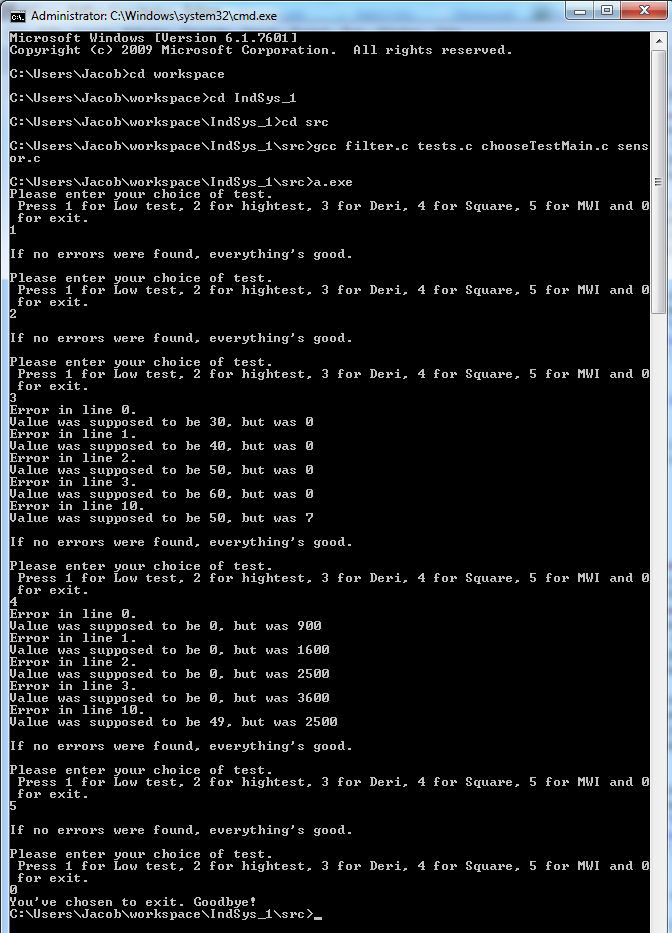
\includegraphics[width=0.5\textwidth]{Results_test.png}
%  \caption{The results of our test cases of the 5 filters.}
\end{figure}
\subsection{Test results of RPeakDetection}

\section{Discussion}
	As mentioned in the critical parts, the processor which the program is tested on is more than powerful enough to fulfil the requirements of 250 data points per second. Therefore, the final processor that is to be used for the ECG scanner should be much less powerful - it makes little sense to use a very powerful processor if it idles most of the time, using power for nothing - and thus, the power consumption will be reduced greatly.\\
	However, if the processor had been too slow, the code could be optimized for speed. To do this, the two functions getIndex and mwInt2 should be examined, as it was determined through a profiler (the GNU Gprof profiler) that it is in these two functions that the most time is spent (see figure \ref{time_result}).\\
	Another way to optimize power would be to use the technical improvements of modern time to make the battery recharge during daily use, for instance by converting the kinetic energy of walking into power for the scanner.\\
	\\
	Regarding the size, the program is generally optimized mostly in terms of speed - currently, an array of 50 data points is used for each filter, but this could be optimized down to using only 2 arrays - one for input, one for output. However, this would also increase the complexity of the task by a great deal and therefore, it was decided to simply use an array for each filter.\\
	\\
	In terms of what should be made as software and what should be put into hardware, it should first be determined which tasks are the most processor-heavy. However, due to the profiler, this is already known - the tasks are getIndex and mwInt2. Therefore, it would also make sense to develop a special processor for these two specific tasks, using a coprocessor for each of these tasks, and a more general-purpose-like processor for the rest of the tasks.\\
	
\subsection{Improvements}
	

\section{Conclusion}
	Implementing the algorithm has been done successfully, enabling the detection of heartbeats according to time and fulfilling all requirements. Furthermore, the processor  used in the final product can easily be downscaled, using a lower clock frequency to reduce power consumption. Finally, all the challenges discovered and discussed in the Theory has been solved.
\newpage
\begin{thebibliography}{9}

\bibitem{lamport94}
  Michael Reibel Boesen, Linas Kaminskas, Paul Pop, Karsten Juul Frederiksen\\
  \emph{Assignment 1: Software implementation of a personal ECG scanner}\\
  3rd Edition\\
  2013.

\bibitem{power consumption}
	http://www.notebookcheck.net/Intel-Core-i7-2630QM-Notebook-Processor.41483.0.html\\
	Date of use: 25/09/2013
\end{thebibliography}
	
\newpage	
	\begin{Large}
		\textbf{Appendix}
	\end{Large}
	\appendix

\section{Who wrote what}
Jacob Gjerstrup, s113440 wrote: Abstract, Introduction, Theory, Discussion (50\%), Conclusion\\
Jakob Welner, s124305 wrote: Design, Implementation, Results, Discussion (50\%)\\

\section{Output of the RPeakDetection}
	\lstinputlisting{output.txt}

	
\section{Sourcecode - introductionary exercises}
\subsection{ReadFromFile}
	Below is the sourcecode for the introductionary-exercise (From september the 4th) - more precisely, the ReadFromFile source-code.\\
	\\
	\lstinputlisting[language=C]{Code/Exercise/main.c}

\subsection{HelloWorld}
	The next is the sourcecode from the same exercise - this time, it's the sourcecode of our HelloWorld program.\\
	\\
	\lstinputlisting{Code/Exercise/HelloWorld.c}
	
\section{Sourcecode - the real program}
	Below follows the sourcecode for each of the parts of our program, split into sections. The first part, the program, is where the various functions are called, and all our data is stored. The Filter.c contains the 5 different filters. The RPeakDetection contains the detection of each peak, along with the calculations of the various thresholds. The sensor is what scans data from the file, and thus simulates that we scan the patient, and finally, the header files is what contains all the prototypes for our functions.
\subsection{Buffer}
	\lstinputlisting[language=C]{Code/buffer.c}	
\subsection{Filters}
	\lstinputlisting[language=C]{Code/filter.c}
\subsection{RPeakDetection}
	R-Peak detection consists of two files - peak detection and RR Handling.\\
	Peak detection:\\
	\lstinputlisting[language=C]{Code/peakDetect.c}	
	RR Handling:\\
	\lstinputlisting[language=C]{Code/RRhandling.c}	
\subsection{Sensor}
	\lstinputlisting[language=C]{Code/sensor.c}	
\subsection{Header files}
\subsubsection{sensor.h}
	Below is the first of the header files, called sensor.h. This file contains the prototype for the sensor as well as the peak detection.\\
	\lstinputlisting{Code/sensor.h}
\subsubsection{buffer.h}
	After this one, the next header file called filter.h comes - this file contains the prototypes of the filters as well as for the buffer.\\
	\lstinputlisting{Code/buffer.h}
\subsection{Tests}
%	We decided to do a run of tests, as discussed in the report. Below is the sourcecode for the tests:
\subsection{Tests of RPeakDetection}
%	\lstinputlisting{RPeakTest.c}
\subsubsection{tests}
%	\lstinputlisting{tests.c}
\subsubsection{Main function for test cases}
%	\lstinputlisting{chooseTestMain.c}
\end{document}